\documentclass[border=10pt]{standalone}
\usepackage{tikz}
\usepackage{amsmath}
\usetikzlibrary{positioning, shapes.geometric, shapes.symbols, fit, backgrounds, calc}

\begin{document}
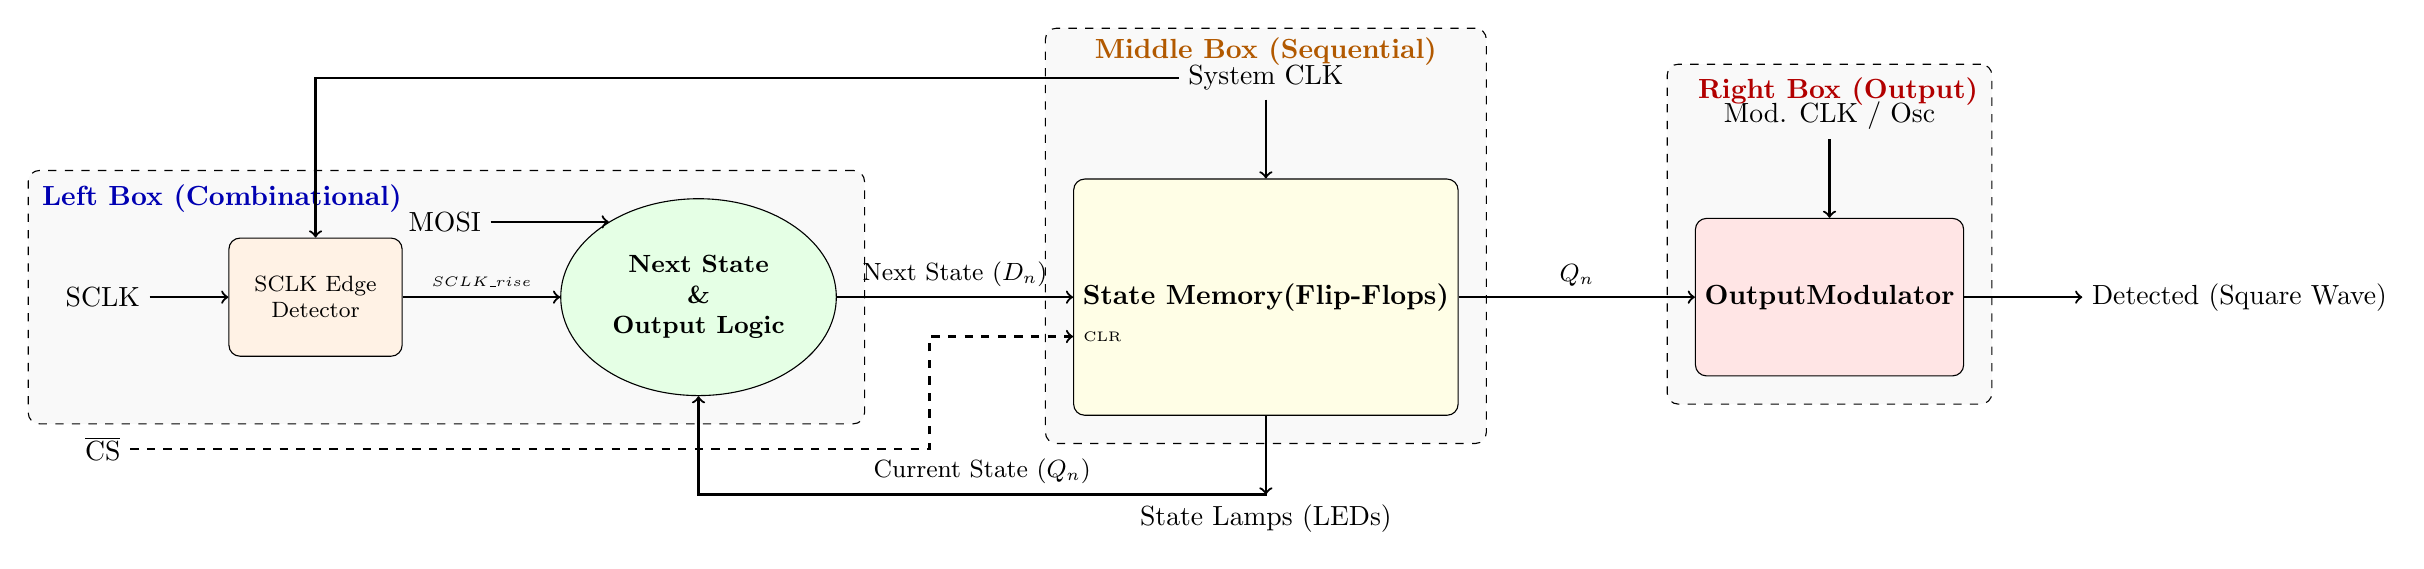
\begin{tikzpicture}
    % Styles
    \tikzset{
        block/.style={rectangle, draw, fill=blue!10, text centered, rounded corners, minimum height=3em, minimum width=4em, font=\bfseries},
        cloud_logic/.style={ellipse, draw, fill=green!10, minimum width=3.5cm, minimum height=2.5cm, align=center, font=\bfseries\small},
        container/.style={draw, dashed, inner sep=1em, rounded corners, fill=gray!5},
        label_text/.style={font=\bfseries\small, align=center}
    }

    % --- Nodes ---

    % Middle Box: State Memory (Flip-Flops)
    \node[block, minimum width=2.5cm, minimum height=3cm, fill=yellow!10] (memory) at (0,0) {State Memory\\(Flip-Flops)};

    % Left Box: Combinational Logic
    \node[cloud_logic, left=3cm of memory] (logic) {Next State\\\&\\Output Logic};

    % Edge Detector
    \node[block, fill=orange!10, left=2.0cm of logic.180, align=center, font=\footnotesize, minimum height=1.5cm, minimum width=2.2cm] (edge_det) {SCLK Edge\\Detector};

    % Right Box: Output Interface
    \node[block, right=3cm of memory, fill=red!10, minimum width=2.5cm, minimum height=2cm] (output_interface) {Output\\Modulator};


    % --- Connections ---

    % Inputs to Logic
    \node[left=1.5cm of logic.140] (mosi) {MOSI};
    \node[left=1.0cm of edge_det] (sclk) {SCLK};
    % CS moved to point to Memory
    \node[below=1.4cm of sclk] (cs) {$\overline{\text{CS}}$};

    \draw[->, thick] (mosi) -- (logic.140);
    \draw[->, thick] (sclk) -- (edge_det);
    \draw[->, thick] (edge_det.east) -- node[above, font=\tiny, sloped] {$SCLK\_rise$} (logic.180);
    
    % Route CS to Memory (Async Clear)
    % Pass under the Logic block
    \draw[->, thick, dashed] (cs) -- ++(10.5,0) |- ([yshift=-5mm]memory.west) node[right, font=\tiny] {CLR};

    % Logic to Memory (Next State D)
    \draw[->, thick] (logic.east) -- node[above, font=\small] {Next State ($D_n$)} (memory.west);

    % Memory to Logic (Feedback Q)
    % We need to route this around
    \draw[->, thick] (memory.south) -- ++(0,-1) -| node[pos=0.25, above, font=\small] {Current State ($Q_n$)} (logic.south);

    % Memory/Logic to Output Interface
    \draw[->, thick] (memory.east) -- node[above, font=\small] {$Q_n$} (output_interface.west);
    
    % Clock to Memory
    \node[above=1cm of memory] (clk) {System CLK};
    \draw[->, thick] (clk) -- (memory.north);
    \draw[->, thick] (clk) -| (edge_det.north);

    % Output Interface Inputs
    % Needs modulation clock?
    \node[above=1cm of output_interface] (mod_clk) {Mod. CLK / Osc};
    \draw[->, thick] (mod_clk) -- (output_interface.north);

    % Final Output
    \node[right=1.5cm of output_interface] (detected) {Detected (Square Wave)};
    \draw[->, thick] (output_interface.east) -- (detected);

    % State Lamp
    \node[below=1.0cm of memory] (lamps) {State Lamps (LEDs)};
    \draw[->, thick] (memory.south) ++(0,-0.5) -- (lamps.north);


    % --- Containers (Boxes) ---
    
    \begin{scope}[on background layer]
        % Left Box
        \node[container, fit=(logic) (mosi) (sclk) (edge_det), label={[anchor=north west, font=\bfseries\color{blue!70!black}, inner sep=5pt]north west:Left Box (Combinational)}] (box_left) {};
        
        % Middle Box
        \node[container, fit=(memory) (clk), label={[anchor=north, font=\bfseries\color{orange!70!black}]north:Middle Box (Sequential)}] (box_mid) {};
        
        % Right Box
        \node[container, fit=(output_interface) (mod_clk), label={[anchor=north east, font=\bfseries\color{red!70!black}, inner sep=5pt]north east:Right Box (Output)}] (box_right) {};
    \end{scope}

\end{tikzpicture}
\end{document}
